\documentclass[a4paper]{scrartcl}
\usepackage[utf8]{inputenc}
\usepackage[english]{babel}
\usepackage{graphicx}
\usepackage{lastpage}
\usepackage{pgf}
\usepackage{wrapfig}
\usepackage{fancyvrb}
\usepackage{fancyhdr}
\usepackage{hyperref}
\pagestyle{fancy}

\catcode`\_=\active
\protected\def_#1_{\textit{#1}}

% Create header and footer
\headheight 27pt
\pagestyle{fancyplain}
\lhead{\footnotesize{Network Programming, ID1212}}
\chead{\footnotesize{Non-blocking Sockets}}
\rhead{}
\lfoot{}
\cfoot{\thepage}
\rfoot{}

% Create title page
\title{Assignment 1 - Non-blocking sockets}
\subtitle{Network Programming, ID1212}
\author{Bernardo Gonzalez Riede, begr@kth.se}
\date{\today}

\begin{document}

\maketitle


\section{Introduction}


\begin{itemize}
    \item Server and client have to communicate via blocking TCP connections.
    TCP is a transport protocol for a network, guaranteeing no lost packets iff a connection is established.
    Moreover, it uses a sequence number to ensure delivery in correct order.
    \item The client must not store any data.
    A stateless implementation of the client is preferred.
    \item The client must have a responsive user interface, i.e. being able to type commands while previous ones are still processed.
    This is at least best practice, if not a requirement in all programs.
    \item The server should be able to handle several clients simulteanously.
    Every client has to have its own game which doesn't get affected by other players.
    \item The user interface must be informative.
\end{itemize}


\section{Literature Study}

The main literature for this assignment was a combination of all the videos related to streams and sockets, i.e. streams-, file-handler-prog-example-,
    sockets-, chat-program-part*.webm, and the related source code files.
By studying the example and refering to javadocs the flow and layering coalesced to a fitting picture.
Most importatn concepts obtained:
\begin{itemize}
    \item The layering doesn't imply that in mvc some kind of view is always at the top.
    A more fitting description is _event initiator_, in case of the server the network layer which receives request from the client.
    \item Using an _enum_ provides access to a finite set of constants which hold their own name as value.
    This is even faster than an integer for switching.
    Perfect for entering commands
    \item Observer pattern can be used to prevent upcalls from layers to layers above.
    \item (G)UI can be made responsive using an additional thread for commands with latency, i.e. network communication.
    \item Stream reading can be layered, e.g. a _DataOutputStream_ over a _BufferedOutputStream_ over a _FileOutputStream_.\end{itemize}


\section{Method}

The MVC approach was used to solve this problem. Although a bit overkill, practicing it will payoff over time.
This meant to use various packages and to have high cohesion with low coupling. Additionally upcalls should be avoided.


The project is in pure Java, using the included libraries.
Developing was done in Netbeans.

\section{Result}


Link to public Github repository with codehttps://github.com/MemBernd/ID1212-blockingSockets
\href{https://github.com/MemBernd/ID1212-blockingSockets}{https://github.com/MemBernd/ID1212-blockingSockets}

\subsection{Blocking TCP sockets}

The socket on the client side is created in client.net.ServerConnection on lines 29-31.
For a socket to be able to connect it needs an adress, composed of the host and a port, and a timeout.
The _setSoTimeout()_ sets the time the socket is blocked.
\\The server has its implementation of sockets in server.net.Server on lines 31.
Aftewards it stays in a loop accepting connection.
When it receives a request on the specified port (configured default of 54321), it accept it, receiving an available socket form the OS for further communication.
This socket is passed to _handleClient()_ where timeouts are set.

\subsection{Stateless client}

The information of the game which have to tracked are:
\begin{itemize}
    \item current word trying to guess
    \item progress in guessing the word
    \item attempts left
    \item score
\end{itemize}
The variables are stored in server.model.GameState.
They are defined on lines 18-21.
While the score is initialized at the creation of a client handler, the remaining variables are initialized on lines 15-78 inside _initializeGame()_ which gets called when the user starts a game.

\subsection{Multithreaded client}

Client.view.Interpreter, the class which the user interacts with, extends the _Thread_ class and isstarted by client.startup.Hangman.
It creates a client.controller.Controller which itself creates a client.net.ServerConnection.
This class holds an inner class, at line 56, _Listener_, extending _Runnable_.
On line 35 of client.net.ServerConnection the second thread of every client is created, an instance of _Listener_.

\subsection{Multithreaded server}

The amount of threads of the server is 1 + amount of connected clients.
The startup starts server.net.Server which listens permanently on line 33.
When receiving a request it starts server.net.Handler, an extension to _Thread_.
Since the users don't share any data, everyone having their own thread, a complete mvc, was selected.
Because accepting a request on line 33 creates a new socket for each client, no need for an id or similar was needed to communicate a client with the correct thread.


\subsection{Communication}
Both, client \& server have access to protocol.Constants where some constans, such as the delimiter for the communication are defined.
Since the client doesn't have to process the received messages in any way, it just prints them out.

\subsection{Layering}
The client is divided as follows:
\begin{itemize}
    \item The model is equivalent to the client.net package holding _ServerConnection_.
    \item The controller resides in client.controller.
    \item The view has classes in client.view, the most interesting one being _Interpreter_, the UI.
    \item Client.startup.Hangman is the startup class.
\end{itemize}

On the server side, the layering is quite similar:
\begin{itemize}
    \item Server.model.GameState holds the game's state. Every server side client thread has its own.
    \item Server.controller.Controller is the controller.
    \item Equivalent to a view, in a sense of event driver, is the server.net package.
    It contains _Server_ and (client)_Handler_.
\end{itemize}

To avoid a upcalls from client.net.ServerConnection to the view, client.net.OutputHandler has been created.
The previously mentioned _Listener_ thread expects such a class as argument when instancing.
The client.view.Interpreter has an extending class to _OutputHandler_ as a inner class which gets passed through the controller to ServerConnection.
Since its a specialization, it can used wherever its superclass can be used.
This enables it to print output without making an call to the view.

\subsection{Informative UI}
In Figure \ref{fig:ui} several of the information provided to the user and his input can be seen.
The instructions at the start of the client, establishing a connection, starting a game, doing a correct (lucky) input and an incorrect one.

\begin{figure}[h!]
  \begin{center}
    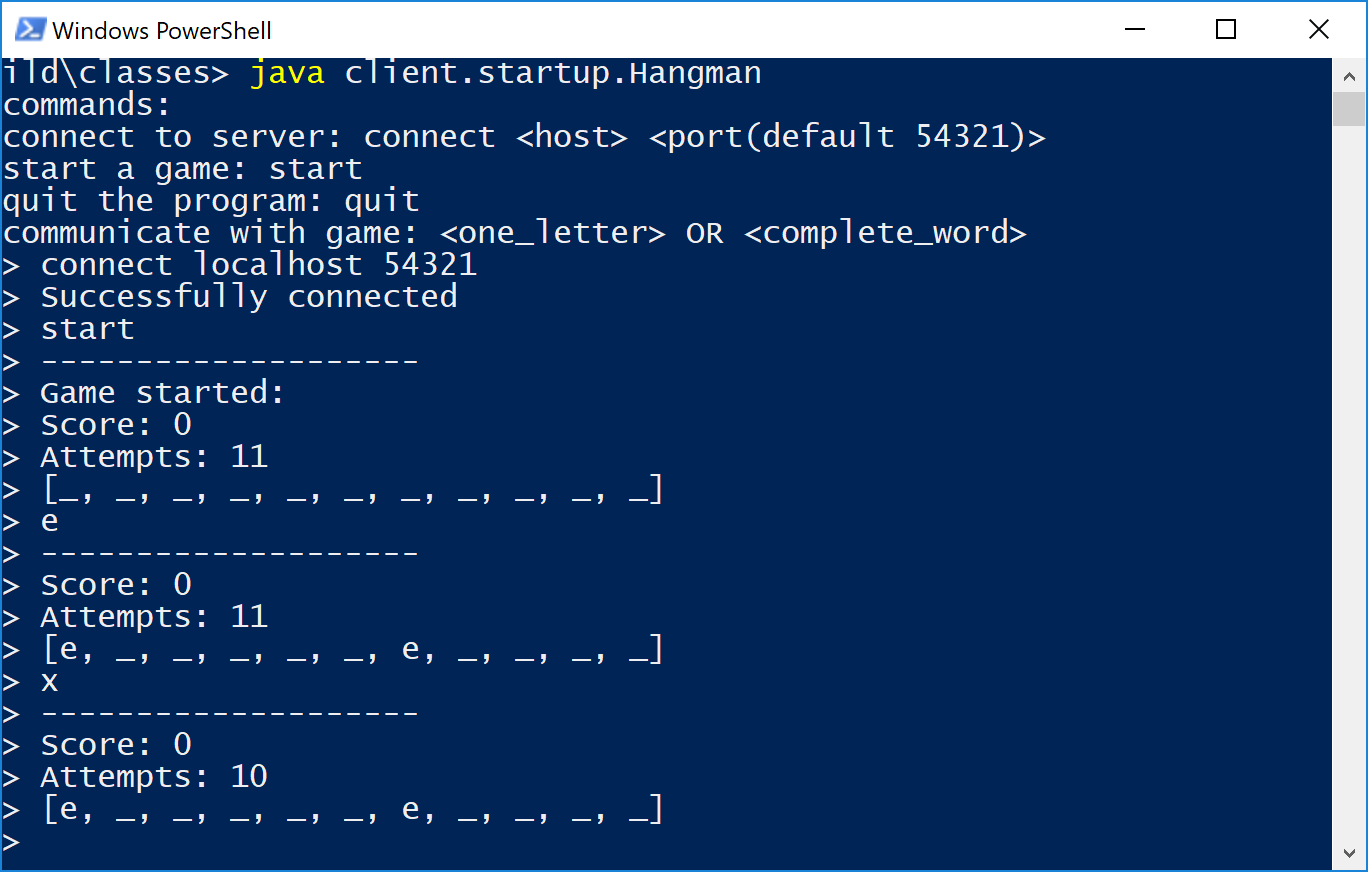
\includegraphics[scale=0.8]{ui.png}
    \caption{Instructions and game state on client side}
    \label{fig:ui}
  \end{center}
\end{figure}

Figure \ref{fig:multiple} shows 2 clients playing at once. Moreover, the timeout used can be seen on the server thread in the right bottom command line.

\begin{figure}[h!]
  \begin{center}
    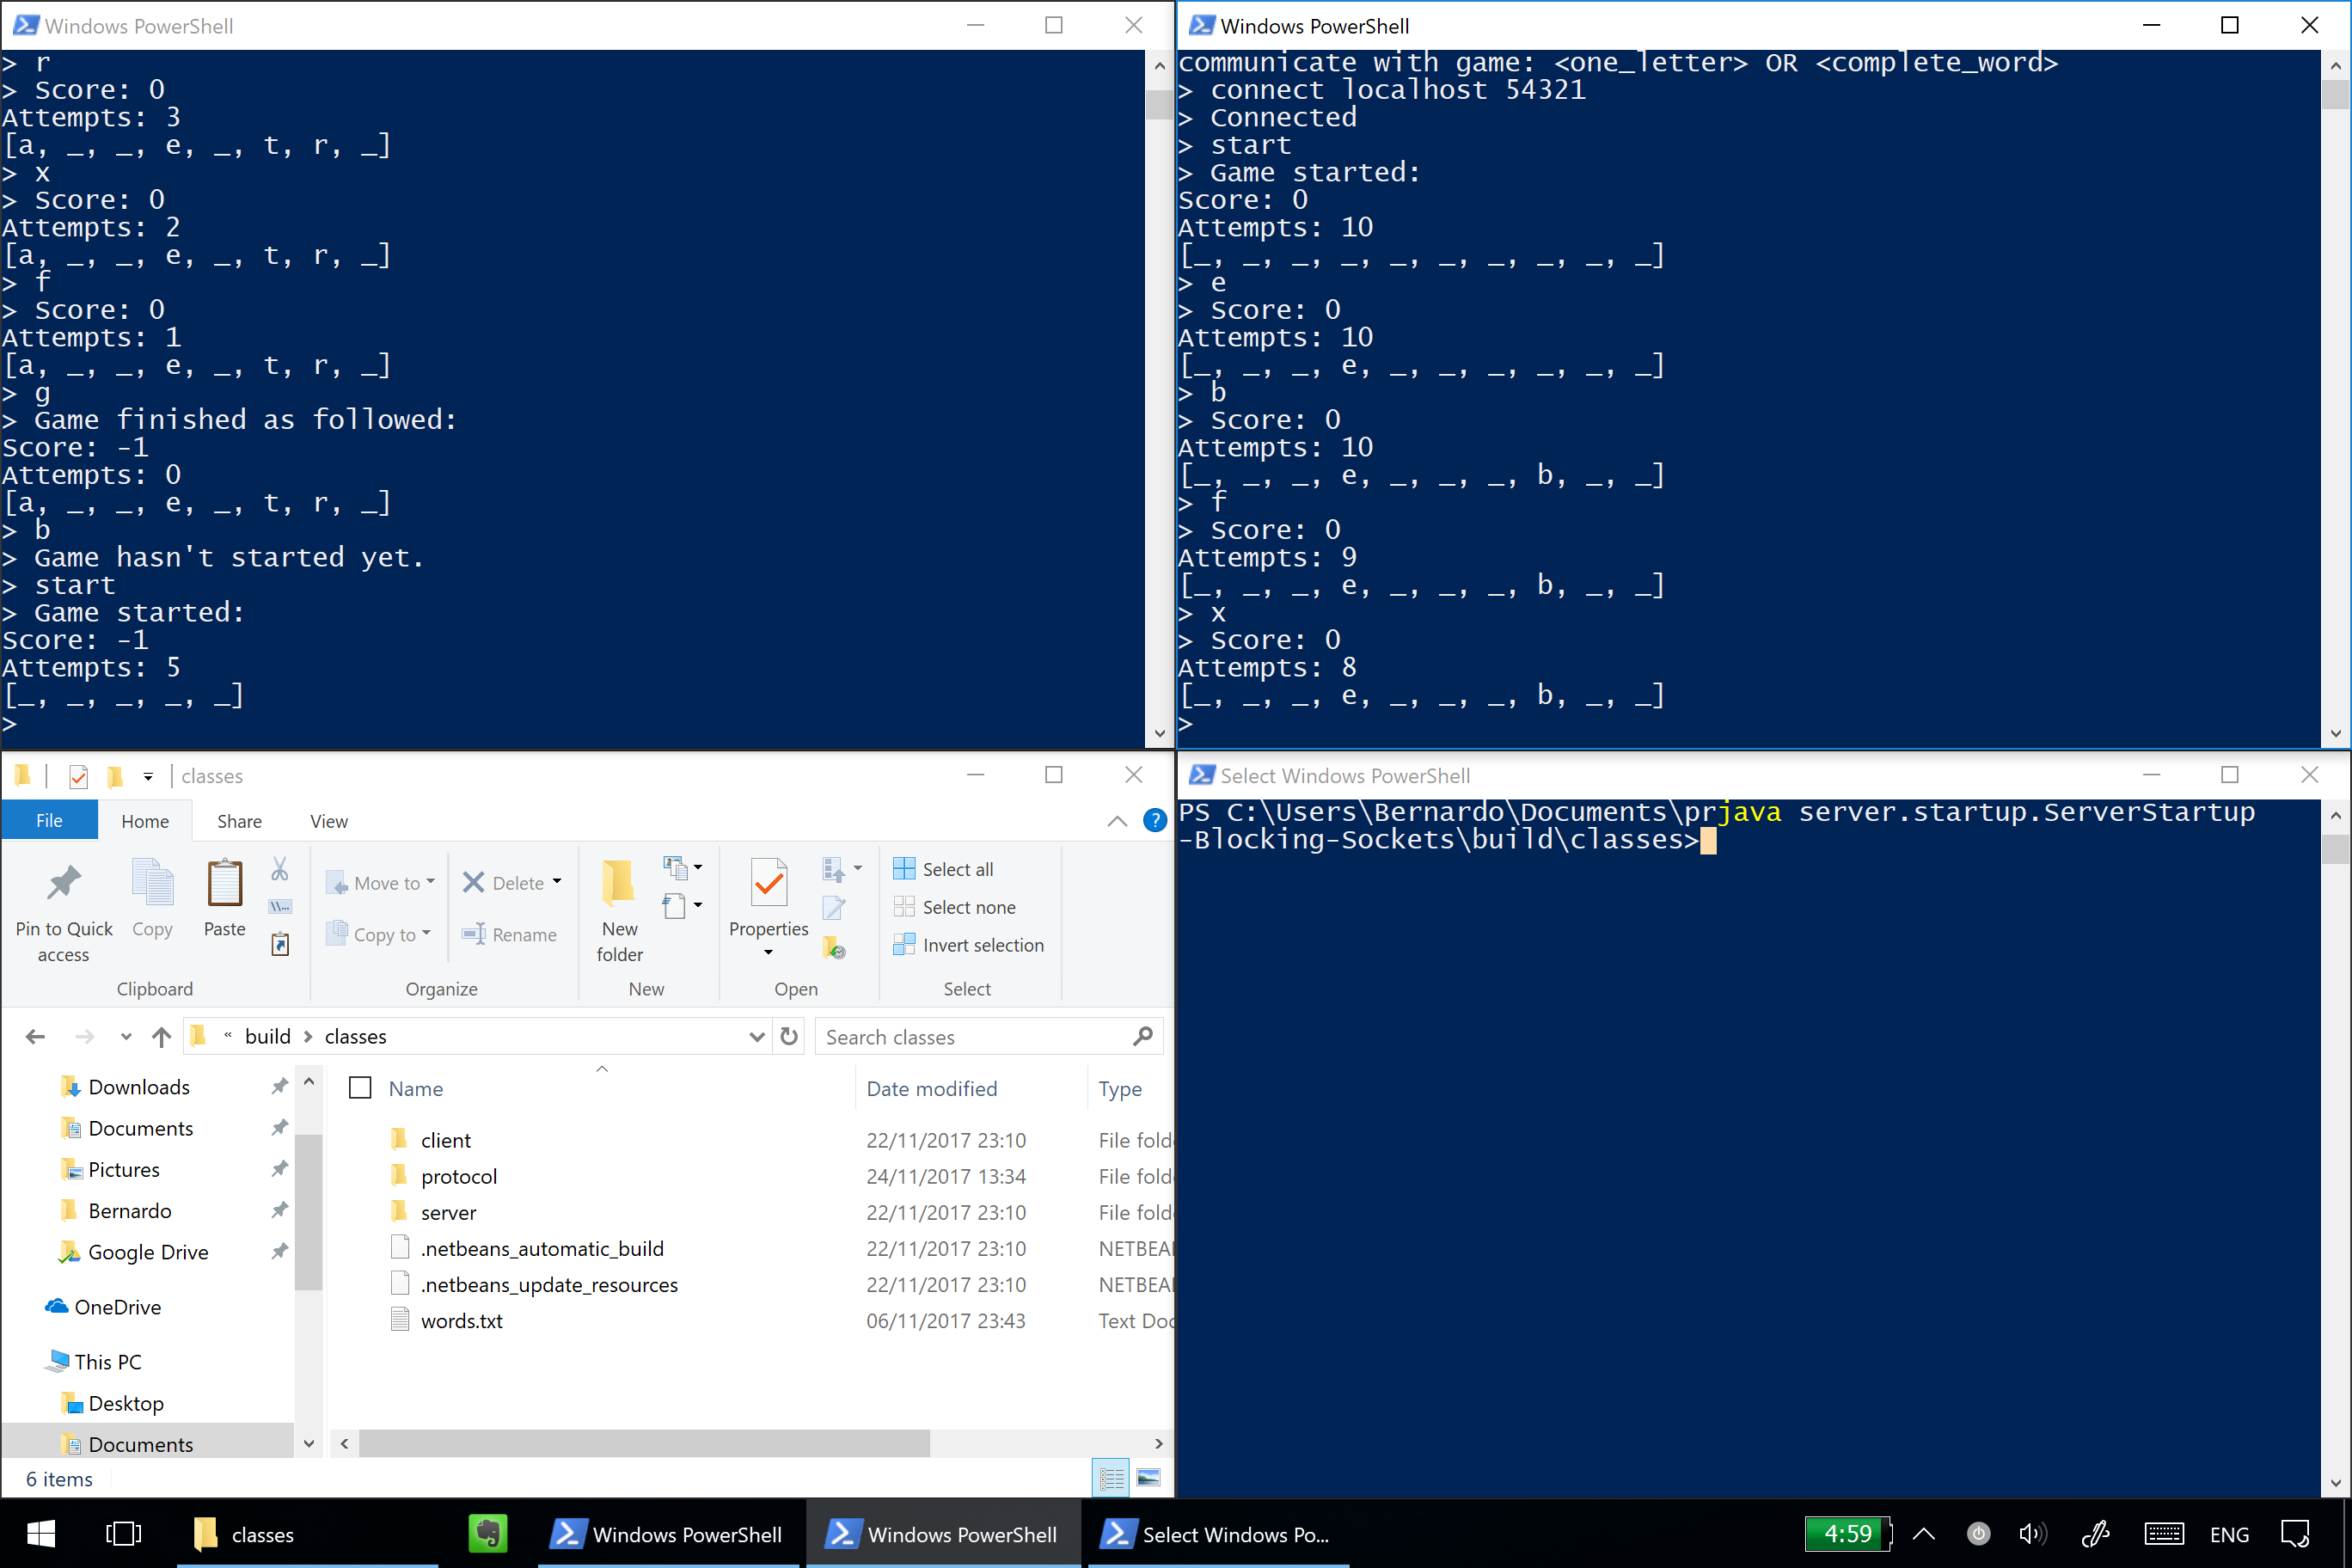
\includegraphics[scale=0.4]{multiple.png}
    \caption{Concurrent players.}
    \label{fig:multiple}
  \end{center}
\end{figure}

\section{Discussion}

All requirements have been met.
Difficulties, once having an understanding, were only encountered regarding on how to use the functions.
It was a lengthy process due to wanting to recreate an elegantly structured program.
At some points the struture of the code itself suffered from it, e.g. server.model.GameState.finishes() needs cleaning.



\section{Comments About the Course}

The code for the sockets is elegant.
Surely enough it creates a bias towards how the implementation can/should be done, resulting in a similar code.
I guess this is why it's mentioned that the copy cannot be copied, though it may be similar.

It took me about 17+-1 hours to do everything, watching videos, planning, coding and writing the report. I tracked the time with toggl.

\end{document}
